\documentclass{beamer}

\usetheme{JuanLesPins}

%\usepackage[utf8]{inputenc}
\usepackage[T1]{fontenc}
\usepackage[french]{babel}
\usepackage[linesnumbered,ruled,french,onelanguage]{algorithm2e}
\usepackage{listings}
\usepackage{color}
\usepackage{pifont}
\usepackage{graphicx}
\newcommand{\umlscale}{0.4}

% Écriture des noms de classes, etc.
\newcommand{\packagename}[1]{\texttt{#1}}
\newcommand{\classname}[1]{\texttt{#1}}
\newcommand{\methodname}[1]{\texttt{#1}}

\definecolor{pblue}{rgb}{0.13,0.13,1}
\definecolor{pgreen}{rgb}{0,0.5,0}
\definecolor{pred}{rgb}{0.9,0,0}

\lstset{language=Python,
  	commentstyle=\color{pgreen},
  	keywordstyle=\color{pblue},
  	stringstyle=\color{pred},
  	basicstyle=\ttfamily,
  	numbers=left,
  	numberstyle=\tiny,
  	basicstyle=\small,
  	frame=single,
  	title=\lstname
}
 
\title{Président}
\date{4 Mai 2022}
\author{Mathieu Goudal, Hugo Bosvy, Valère Sarfati, Edwin Bertin-Cohonner}
\institute{Université de Caen Normandie}

\setbeamertemplate{navigation symbols}{}% pour enlever les symboles de navigation en bas de chaque page
\setbeamertemplate{footline}[frame number]%pour changer le pied de page par un affichage des numéros de slide

\begin{document}

\maketitle

%--------------------
\begin{frame} 
\frametitle{Plan}
\tableofcontents
\end{frame}
%--------------------
\section{Introduction}
\begin{frame}
\frametitle{Projet}
\textbf{Choix du projet}
\begin{center}

\includegraphics[width=5cm]{./img/cartes.png}
\end{center}
\end{frame}

\begin{frame}
\frametitle{Objectifs du projet}

\begin{center}
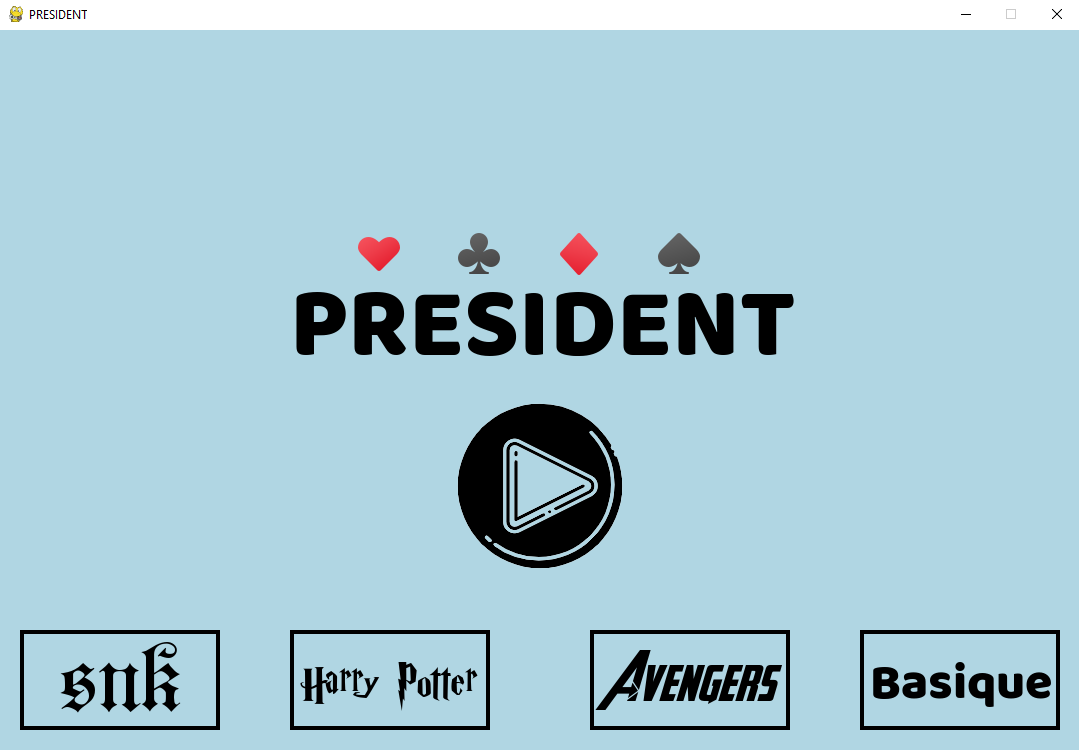
\includegraphics[width=5cm]{./img/accueil.png}
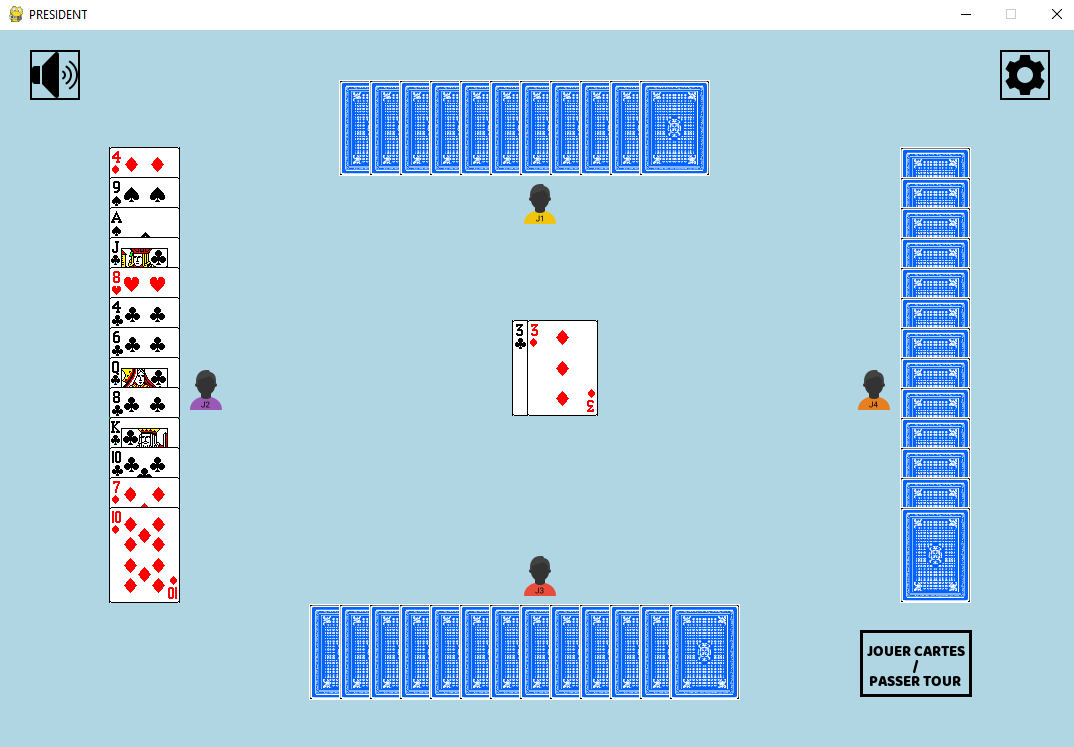
\includegraphics[width=5cm]{./img/cartes_posees.png}
\end{center}

\end{frame}
%--------------------
\section{Gestion des cartes}

\begin{frame}
\frametitle{class$\_$carte}

\begin{center}
  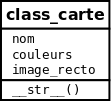
\includegraphics[scale=0.8]{./img/class_carte.png}
\end{center}
\end{frame}

\begin{frame}[containsverbatim]
\frametitle{class$\_$deck}

\begin{lstlisting}[tabsize=4,gobble=4]
	def __init__(self,type=config.DECK_52):
		...
		if type==config.DECK_52: 
            for i in range(1,14):
                for j in Cartes.couleurs:
                    car = Cartes(i+2, Cartes.nom[i], j)
                    self.paquet.append(car)
\end{lstlisting}
\end{frame}

\begin{frame}
\frametitle{class$\_$joueur}

\begin{center}
  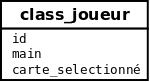
\includegraphics[scale=0.8]{./img/class_joueur.png}
\end{center}
\end{frame}

\section{Gestion du Jeu}
\begin{frame}[containsverbatim]
\frametitle{Création de joueurs}

\begin{lstlisting}[tabsize=4,gobble=4]
	def __init__(self):
		...
		id_joueur=[1,2,3,4]
        for u in id_joueur:
            j = Joueur(u)
            for g in range (0,13):
                carte = self.pioche.tirer()
                j.main.ajouter(carte)
            self.liste_joueur.append(j)
\end{lstlisting}
\end{frame}

\begin{frame}
\frametitle{Fonctions importantes de president.py}

\begin{center}
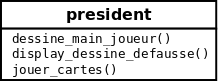
\includegraphics[scale=0.8]{./img/president.png}
\end{center}

\end{frame}

\section{Conclusion}
\begin{frame}
\begin{columns}
\begin{column}{5cm}
Objectifs réalisés
\newline
\begin{itemize}
    \item[\ding{47}] Mode Multijoueurs
 	\item[\ding{47}] Différents choix d'interfaces
 	\item[\ding{47}] Jeu complet
\end{itemize}
\end{column}
\begin{column}{4cm}
Objectifs non-réalisés
\newline
\begin{itemize}
    \item[\ding{47}] Règle du "ta gueule"
 	\item[\ding{47}] Système de relance de partie
 	\item[\ding{47}] Système de points / classement
\end{itemize}
\end{column}
\end{columns}
\end{frame}

\end{document}
